\documentclass[12pt,a4paper]{report}

\usepackage[utf8]{inputenc}
\usepackage[T1]{fontenc}
\usepackage[french,english]{babel}
\usepackage{geometry}
\usepackage{graphicx}
\usepackage{booktabs}
\usepackage{longtable}
\usepackage{array}
\usepackage{hyperref}
\usepackage{float}
\usepackage{setspace}
\usepackage{titlesec}
\usepackage{caption}
\usepackage{xcolor}
\usepackage{enumitem}

\geometry{margin=2.5cm}
\onehalfspacing
\hypersetup{
    colorlinks=true,
    linkcolor=blue,
    urlcolor=blue,
    citecolor=blue
}

\titleformat{\chapter}[display]
{\normalfont\bfseries\Huge}
{\chaptertitlename\ \thechapter}{20pt}{\Huge}

\begin{document}

\selectlanguage{french}

% =========================================================
% PAGE DE GARDE
% =========================================================
\begin{titlepage}
    \centering
    \vspace*{1cm}
    {\Large Paris School of Technology \& Business \par}
    \vspace{0.5cm}
    {\large Mast\`ere Data Science in Business \par}
    \vspace{2cm}
    {\Huge\bfseries Detection de fraude dans la banque digitale par une approche hybride Self-Supervised Learning et XGBoost \par}
    \vspace{1cm}
    {\Large Professional Capstone - Memoire de fin d'annee \par}
    \vspace{2cm}
    \begin{flushleft}
    \textbf{Etudiants :} Nom Prenom 1, Nom Prenom 2\\
    \textbf{Encadrant :} A completer\\
    \textbf{Annee universitaire :} 2025-2026\\
    \textbf{Ecole :} PST\&B - Paris School of Technology \& Business
    \end{flushleft}
    \vfill
    {\large Version 1 - Document de travail \par}
\end{titlepage}

% =========================================================
% RESUMES
% =========================================================
\chapter*{Resume}
\addcontentsline{toc}{chapter}{Resume}

Ce memoire traite de la detection de fraude dans la banque digitale a partir de donnees transactionnelles fortement desequilibrees. Le projet propose une demarche hybride combinant exploration par self-supervised learning, apprentissage supervise et optimisation metier. Le dataset IEEE-CIS Fraud Detection est utilise comme base experimentale principale. Apres plusieurs iterations de preprocessing, de modelisation et de comparaison, le modele final retenu est un XGBoost optimise, associe a un seuil de decision metier. Les resultats obtenus montrent une performance elevee avec une AUC-ROC de 0,9718, une Average Precision de 0,8608, un F1-score de 0,8210, une precision de 0,8797 et un recall de 0,7697. Le projet integre egalement des KPIs business, une estimation d'impact financier et un dashboard Streamlit deploye afin de rendre les resultats exploitables par une banque digitale.

\textbf{Mots cles :} fraude bancaire, banque digitale, XGBoost, self-supervised learning, KPIs metier.

\chapter*{Abstract}
\addcontentsline{toc}{chapter}{Abstract}

This thesis addresses fraud detection in digital banking using highly imbalanced transactional data. The project follows a hybrid approach combining self-supervised learning exploration, supervised learning and business-oriented threshold optimization. The IEEE-CIS Fraud Detection dataset is used as the main experimental benchmark. After several iterations of preprocessing, modelling and comparison, the final retained model is an optimized XGBoost classifier associated with a business decision threshold. The final results show strong performance, with an ROC-AUC of 0.9718, an Average Precision of 0.8608, an F1-score of 0.8210, a precision of 0.8797 and a recall of 0.7697. The project also includes business KPIs, financial impact estimation and a deployed Streamlit dashboard to make the results understandable and actionable for digital banking stakeholders.

\textbf{Keywords:} banking fraud, digital banking, XGBoost, self-supervised learning, business KPIs.

\chapter*{Remerciements}
\addcontentsline{toc}{chapter}{Remerciements}

Nous tenons a remercier l'equipe pedagogique de PST\&B pour l'accompagnement apporte dans le cadre du Mast\`ere Data Science in Business. Ce projet a permis de mobiliser des competences techniques en data science, machine learning et visualisation, tout en les reliant a une problematique business concrete. Nous remercions egalement les personnes ayant contribue aux echanges, aux tests et a la validation progressive de la demarche experimentale.

\tableofcontents
\listoffigures
\listoftables

\chapter*{Glossaire et abreviations}
\addcontentsline{toc}{chapter}{Glossaire et abreviations}

\begin{longtable}{p{3cm}p{11cm}}
\toprule
\textbf{Terme} & \textbf{Definition} \\
\midrule
SSL & Self-Supervised Learning, methode d'apprentissage qui exploite les donnees non labellisees en construisant une tache auxiliaire. \\
XGBoost & Algorithme de gradient boosting base sur des arbres de decision, performant sur donnees tabulaires. \\
PR-AUC & Aire sous la courbe precision-recall, utile pour les donnees desequilibrees. \\
AUC-ROC & Aire sous la courbe ROC, mesure globale de capacite de discrimination. \\
Recall & Part des fraudes reelles detectees par le modele. \\
Precision & Part des alertes du modele qui correspondent réellement a des fraudes. \\
F1-score & Moyenne harmonique entre precision et recall. \\
Faux positif & Transaction legitime signalee a tort comme suspecte. \\
Faux negatif & Fraude reelle non detectee par le modele. \\
ETL & Extract, Transform, Load : chaine de preparation des donnees. \\
KPI & Key Performance Indicator, indicateur cle de performance. \\
\bottomrule
\end{longtable}

% =========================================================
% INTRODUCTION EN ANGLAIS
% =========================================================
\selectlanguage{english}
\chapter{Introduction}

\section{Context and motivation}

Digital banking has profoundly transformed the way financial services are delivered. Customers can now open accounts, make payments, transfer money, use cards, access credit services and interact with financial institutions through digital channels. This transformation creates major opportunities for banks: faster services, lower operational costs, better customer experience and large-scale data collection. However, it also increases exposure to fraud. Fraudsters can exploit online payment systems, stolen credentials, card-not-present transactions, automated attacks and identity weaknesses to generate financial losses.

Fraud detection is therefore a strategic issue for digital banks. The objective is not only to identify suspicious transactions, but also to do so in a way that is operationally usable. A model that detects many frauds but generates too many false alerts can overload investigation teams and damage customer experience. Conversely, a model that is too conservative may miss fraudulent transactions and create direct financial losses. This trade-off makes fraud detection both a technical and a business problem.

The project is developed within the Master in Data Science in Business at PST\&B. The programme emphasizes the ability to exploit, analyze and interpret data through statistical, mathematical and algorithmic tools in order to support business strategy. In this perspective, this thesis does not aim to build a model in isolation. It aims to design an end-to-end decision-support system for digital banking fraud detection, combining data preparation, machine learning, business KPIs, threshold optimization and interactive visualization.

\section{Research problem}

Fraud detection in digital banking presents several challenges. First, fraud is rare compared with legitimate transactions. In the IEEE-CIS Fraud Detection dataset used in this project, only 3.50\% of transactions are fraudulent. This class imbalance makes accuracy misleading and requires more adapted metrics such as precision, recall, F1-score and Average Precision. Second, fraud patterns are complex and may evolve over time. Fraudulent transactions can imitate legitimate behavior, making detection difficult. Third, business constraints must be considered: false positives create investigation costs and customer friction, while false negatives create financial losses.

The central research question of this thesis is therefore:

\begin{quote}
How can a hybrid digital banking fraud detection system, combining self-supervised learning, supervised learning and business optimization, improve performance, explainability and decision usability in a highly imbalanced data context?
\end{quote}

\section{Methodological approach}

The project follows an empirical and iterative methodology. The starting point is a real-world-inspired transactional dataset, IEEE-CIS Fraud Detection, which provides a large volume of transactions and a binary fraud label. The first phase consists in understanding the data, identifying its structure, missing values, imbalance and business variables. The second phase consists in building an ETL-like preprocessing pipeline to transform raw CSV files into model-ready datasets.

The modelling phase explores self-supervised learning through a masked-feature reconstruction approach. The purpose is to assess whether a neural encoder can learn useful transaction representations without relying directly on fraud labels. These representations are then compared with supervised models. The experiments show that, on this tabular dataset, XGBoost remains more effective than the SSL embeddings for final classification. The final model is therefore an optimized XGBoost classifier trained on the improved preprocessing version.

The final phase translates model outputs into business value. The selected model is evaluated not only through machine learning metrics, but also through financial and operational KPIs: number of frauds detected, false alerts, investigation cost, saved amount and estimated net benefit. A Streamlit dashboard is deployed to present the results and provide a transaction testing interface and a business assistant.

\section{Contributions}

This thesis contributes to the project in four main ways. First, it provides a structured pipeline for preparing and modelling digital transaction data. Second, it evaluates the role of self-supervised learning in a tabular fraud detection context and discusses its limits. Third, it proposes an optimized XGBoost model with strong final performance. Fourth, it translates technical results into business indicators and an operational dashboard, making the model understandable for non-technical stakeholders.

\section{Structure of the thesis}

The thesis is organized as follows. Chapter 2 presents the literature review on digital banking fraud detection, imbalanced classification, self-supervised learning and model evaluation. Chapter 3 describes the dataset and justifies its relevance for a Data Science in Business project. Chapter 4 details the methodology, including ETL, preprocessing, SSL experiments, XGBoost modelling and threshold selection. Chapter 5 presents the experimental results and business KPIs. Chapter 6 discusses the dashboard and assistant system. Chapter 7 provides operational recommendations. The conclusion summarizes the contributions, limitations and future perspectives.

% =========================================================
% LITERATURE REVIEW EN ANGLAIS
% =========================================================
\chapter{Literature Review}

\section{Fraud detection in digital banking}

Fraud detection is a critical function in digital financial services. With the growth of online banking, e-commerce payments, mobile transactions and card-not-present operations, banks and payment platforms face increasing pressure to detect fraudulent behavior quickly and accurately. Fraud detection is not only a data science problem: it is also connected to operational risk, customer trust, regulatory expectations and financial performance.

The literature on credit card fraud detection highlights several structural characteristics of the problem. Lucas and Jurgovsky \cite{lucas2020survey} describe credit card fraud detection as a specialized machine learning task involving transactional attributes, cardholder-related attributes, merchant-related information and fraud labels. They emphasize that real transaction data are highly sensitive and rarely available publicly, which makes public benchmarks valuable for reproducible research.

Fraud detection systems must also deal with evolving behaviors. Fraudsters adapt their strategies, while legitimate customers also change their purchasing habits over time. This creates potential dataset shift and concept drift. A model trained on historical data may lose relevance if fraud patterns change. Although this thesis does not implement an online learning system, the issue supports the need for periodic monitoring and retraining.

\section{Class imbalance and evaluation metrics}

A central challenge in fraud detection is class imbalance. Fraudulent transactions represent a small minority of the total number of transactions. In such contexts, accuracy can be misleading: a model that predicts all transactions as legitimate may achieve high accuracy while detecting no fraud. For this reason, metrics such as precision, recall, F1-score, ROC-AUC and PR-AUC are more relevant.

Precision measures the proportion of predicted fraud alerts that are truly fraudulent. Recall measures the proportion of actual frauds detected by the model. F1-score combines both dimensions. These metrics directly reflect operational trade-offs. High recall reduces missed frauds but may increase false positives. High precision reduces false alerts but may miss more frauds.

Saito and Rehmsmeier \cite{saito2015pr} show that Precision-Recall curves are particularly informative for imbalanced classification. In such contexts, ROC curves can sometimes give an overly optimistic impression because they are less sensitive to class prevalence. This is why the project uses Average Precision as a key optimization metric during hyperparameter tuning.

\section{Machine learning models for tabular fraud detection}

Traditional machine learning models remain widely used for fraud detection. Logistic regression, decision trees, random forests, gradient boosting, support vector machines and neural networks are commonly evaluated. In structured transactional data, tree-based models are often strong baselines because they can handle non-linear interactions, missingness patterns and heterogeneous variables after preprocessing.

XGBoost is particularly suited to tabular data. It combines gradient boosting, regularization and efficient tree construction. It also allows class imbalance handling through the `scale\_pos\_weight` parameter, which increases the relative importance of fraud examples during training. In this project, XGBoost progressively became the final supervised model because it outperformed the neural SSL-based classifier on validation metrics.

Recent work on imbalanced fraud detection confirms that gradient-boosted tree models remain highly competitive. Han and Wu \cite{han2026cfa} use IEEE-CIS as a benchmark and note that strong gradient-boosted tree models already perform well on structured transaction data. This supports the empirical observation made in this project.

\section{Self-supervised learning and limited labels}

Self-supervised learning aims to learn useful representations from unlabeled data by solving an auxiliary task. In computer vision, this may involve predicting missing image patches or contrasting augmented views. In natural language processing, masked token prediction is a common strategy. In tabular fraud detection, a possible SSL task is masked-feature reconstruction: some variables of a transaction are hidden, and the model learns to reconstruct them from the remaining variables.

The motivation for testing SSL is linked to the cost of fraud labels. Deng and Ruan \cite{deng2019fraudjudger} argue that manually labeled fraud data can be difficult and costly to obtain, while unlabeled transaction data are abundant in digital payment platforms. This supports the relevance of exploring representation learning approaches.

However, the literature also suggests that tabular data differ from images and text. Many tabular variables are already engineered or structured, and tree-based supervised models can exploit them directly. The experiments in this project confirm this limitation: SSL helped structure the research approach, but it did not outperform XGBoost on the final classification task.

\section{Business evaluation and decision thresholds}

Fraud detection models output probabilities or risk scores. The final decision depends on a threshold. A low threshold increases recall but creates more alerts; a high threshold increases precision but misses more frauds. Therefore, threshold selection is a business decision, not only a technical one.

In banking operations, the cost of a false negative is generally the financial loss of an undetected fraud, while the cost of a false positive is the operational cost of investigation and the potential customer friction. This explains why the final system must include threshold analysis, cost estimation and business KPIs. The model must be evaluated as part of a decision process.

\section{Positioning of this thesis}

This thesis is positioned at the intersection of machine learning, digital banking risk and business decision support. It does not only compare algorithms. It builds an applied pipeline where data preparation, modelling, evaluation, threshold optimization and dashboard deployment are connected. This is consistent with the Data Science in Business orientation of PST\&B, where data science is used to support strategic and operational decisions.

\selectlanguage{french}

% =========================================================
% CHAPITRE 3
% =========================================================
\chapter{Contexte professionnel et choix du dataset}

\section{Contexte de la banque digitale}

La banque digitale repose sur la dematerialisation des services financiers. Les clients peuvent effectuer des paiements, consulter leurs comptes, utiliser des cartes, realiser des transferts et interagir avec leur banque sans passage physique en agence. Cette transformation augmente le volume de donnees disponibles et permet l'automatisation de nombreuses decisions. En contrepartie, elle expose les banques a de nouveaux risques : usurpation d'identite, fraude carte, fraude en ligne, compromission de comptes, transactions suspectes et comportements automatises.

Dans ce contexte, la detection de fraude est un enjeu central. Une banque digitale doit identifier rapidement les transactions suspectes afin de reduire les pertes financieres, tout en maintenant une experience client fluide. Une solution trop agressive peut bloquer des clients legitimes, generer des plaintes et augmenter les couts d'investigation. Une solution trop permissive peut laisser passer des fraudes couteuses. Le projet doit donc repondre a un double objectif : performance predictive et exploitabilite metier.

\section{Problematique retenue}

La problematique retenue est la suivante :

\begin{quote}
Comment concevoir un systeme hybride de detection de fraude bancaire digitale, combinant self-supervised learning, apprentissage supervise et optimisation metier, afin d'ameliorer la performance, l'explicabilite et l'exploitabilite des decisions dans un contexte de donnees fortement desequilibrees ?
\end{quote}

Cette problematique exprime trois dimensions. La premiere est technique : il faut construire un modele capable d'identifier les fraudes dans un jeu de donnees desequilibre. La deuxieme est scientifique : il faut tester l'interet du self-supervised learning dans un contexte ou les labels peuvent etre limites. La troisieme est business : il faut transformer les scores du modele en decisions et indicateurs utiles pour une banque digitale.

\section{Justification du choix du dataset}

Le dataset principal retenu est IEEE-CIS Fraud Detection, publie sur Kaggle dans le cadre d'une competition associee a l'IEEE Computational Intelligence Society et a Vesta, acteur specialise dans la prevention de fraude sur les paiements digitaux. Il contient des transactions numeriques avec un label binaire de fraude.

Ce choix se justifie d'abord par son adequation au contexte bancaire digital. Le dataset contient des variables relatives au montant, au produit, a la carte, aux emails, au temps et aux informations d'identite ou de device. Cette structure correspond a une logique de monitoring transactionnel, ou chaque transaction doit etre evaluee en fonction de son niveau de risque.

Le dataset se justifie ensuite par son desequilibre. Il contient 590 540 transactions, dont 20 663 fraudes, soit un taux de fraude de 3,50\%. Cette rarete reproduit une contrainte centrale des systemes bancaires reels : les transactions frauduleuses sont minoritaires, mais elles portent un impact financier important. Cette caracteristique justifie l'utilisation de metriques adaptees telles que le recall, la precision, le F1-score et la PR-AUC.

Enfin, le dataset offre une richesse metier. Contrairement a certains jeux de donnees de fraude carte entierement anonymises par PCA, IEEE-CIS conserve des variables interpretables ou semi-interpretables. Cela permet de produire des KPIs metier : taux de fraude par produit, volume frauduleux, risque par type de carte, risque par heure, cout d'investigation et benefice net estime.

\section{Description des fichiers}

\begin{table}[H]
\centering
\caption{Fichiers principaux du dataset IEEE-CIS}
\begin{tabular}{p{5cm}p{4cm}p{5cm}}
\toprule
\textbf{Fichier} & \textbf{Role} & \textbf{Description} \\
\midrule
train\_transaction.csv & Donnees transactionnelles d'entrainement & 590 540 lignes, contient le label `isFraud`. \\
train\_identity.csv & Donnees d'identite & Informations device et identite disponibles pour une partie des transactions. \\
test\_transaction.csv & Donnees transactionnelles de test & Transactions sans label cible. \\
test\_identity.csv & Identite test & Donnees identity associees au test. \\
sample\_submission.csv & Format Kaggle & Exemple de soumission. \\
\bottomrule
\end{tabular}
\end{table}

\section{Pertinence pour PST\&B Data Science in Business}

Le projet s'inscrit directement dans l'esprit du Mast\`ere Data Science in Business de PST\&B. Il ne s'agit pas uniquement de produire un modele performant, mais de transformer un probleme de risque financier en dispositif d'aide a la decision. La demarche combine exploitation de donnees, algorithmes, interpretation metier, KPIs et visualisation interactive.

La finalite est donc double : demontrer une competence technique en data science et montrer comment cette competence peut orienter une strategie operationnelle dans une organisation bancaire digitale.

% =========================================================
% CHAPITRE 4
% =========================================================
\chapter{Methodologie}

\section{Vue d'ensemble de la demarche}

La demarche adoptee est empirico-inductive. Le point de depart est un phenomene professionnel concret : la difficulte de detecter la fraude dans un environnement bancaire digital. A partir de ce phenomene, le projet construit un pipeline experimental permettant de tester plusieurs approches, d'analyser les resultats, puis de formuler une solution operationnelle.

La methodologie suit sept etapes principales :

\begin{enumerate}
    \item comprehension du dataset et analyse exploratoire ;
    \item construction d'un ETL leger ;
    \item preprocessing V1 et identification des limites ;
    \item preprocessing V2 enrichi ;
    \item experimentation self-supervised learning ;
    \item comparaison avec XGBoost et optimisation ;
    \item traduction des resultats en KPIs business et dashboard.
\end{enumerate}

\section{ETL leger}

Un data warehouse complet n'a pas ete retenu, car le projet repose sur un dataset fixe et non sur des flux de donnees continus. En revanche, un ETL leger a ete mis en place afin de garantir une preparation reproductible des donnees.

La phase Extract consiste a charger les fichiers CSV et a joindre les tables transaction et identity via la cle `TransactionID`. La phase Transform applique le nettoyage, l'imputation, l'encodage et la creation de features. La phase Load sauvegarde les donnees nettoyees en format Parquet, plus leger et plus rapide a charger que les CSV bruts.

\section{Preprocessing V1}

La premiere version du preprocessing visait a obtenir rapidement un dataset exploitable. Elle supprimait les colonnes contenant plus de 70\% de valeurs manquantes, imputait les valeurs manquantes numeriques par la mediane, remplacait les categories manquantes par `UNKNOWN`, encodait les variables categorielles et normalisait les variables numeriques.

Cette version a permis d'entrainer les premiers modeles, mais elle a revele une limite importante : le seuil de 70\% etait trop strict. Il supprimait de nombreuses variables potentiellement informatives, notamment certaines variables anonymisees Vesta. De plus, l'imputation simple pouvait effacer le signal porte par l'absence d'information.

\section{Preprocessing V2}

La deuxieme version du preprocessing corrige ces limites. Le seuil de suppression des colonnes a ete releve a 95\%, ce qui permet de conserver beaucoup plus de variables. Des indicateurs de valeurs manquantes ont ete ajoutes afin que le modele puisse exploiter le fait qu'une information soit absente. Des features temporelles ont ete creees a partir de `TransactionDT`, notamment l'heure de transaction et les periodes de pic de fraude.

Cette evolution a fait passer le nombre de variables finales a environ 743 features. Elle constitue une etape majeure du projet, car elle montre une demarche iterative : les premiers resultats ont ete analyses, les limites ont ete identifiees, puis le preprocessing a ete ameliore.

\section{Self-supervised learning}

Le self-supervised learning a ete teste a travers une logique de reconstruction de features masquees. Pour chaque transaction, une partie des variables est masquees aleatoirement. Le modele doit ensuite reconstruire les valeurs cachees a partir des autres variables. Cette tache ne necessite pas le label `isFraud`, ce qui correspond au principe du SSL.

L'objectif etait de verifier si un encodeur pouvait apprendre une representation generale des transactions, puis aider la detection de fraude avec peu de labels. Cette approche est pertinente en theorie, car dans la realite bancaire, les labels de fraude sont couteux a obtenir et dependent d'investigations humaines.

Les resultats ont toutefois montre que, dans ce dataset tabulaire, les embeddings SSL n'apportaient pas de gain significatif par rapport aux features originales exploitees par XGBoost. Ce resultat negatif n'a pas ete cache : il constitue une conclusion scientifique importante du projet. Le SSL a permis d'explorer une hypothese, mais le modele final operationnel repose sur XGBoost.

\section{XGBoost et optimisation}

XGBoost a ete retenu comme modele final pour plusieurs raisons. Il est performant sur donnees tabulaires, robuste aux interactions non lineaires, compatible avec la gestion du desequilibre des classes et efficace en temps d'entrainement. Le parametre `scale\_pos\_weight` a ete utilise pour tenir compte du ratio entre transactions legitimes et frauduleuses.

Une optimisation d'hyperparametres a ensuite ete realisee. La metrique optimisee est l'Average Precision, car elle est mieux adaptee a un contexte desequilibre que l'accuracy. Les hyperparametres finaux retenus incluent notamment une profondeur maximale de 9, un learning rate de 0,1487, 562 estimateurs, ainsi qu'une regularisation `reg\_alpha` et `reg\_lambda`.

\section{Choix du seuil de decision}

Un modele de fraude produit un score de risque. Le seuil transforme ce score en decision : fraude ou non fraude. Le choix du seuil influence directement le recall, la precision et le nombre de fausses alertes. Dans ce projet, le seuil final retenu est 0,56, car il maximise le compromis metrique obtenu sur validation apres optimisation du modele.

Ce seuil permet d'obtenir une precision de 0,8797 et un recall de 0,7697. Il est donc coherent avec une logique bancaire : detecter une part importante des fraudes tout en gardant un volume de fausses alertes operationnellement acceptable.

% =========================================================
% CHAPITRE 5
% =========================================================
\chapter{Resultats experimentaux}

\section{Progression des iterations}

La demarche experimentale s'est construite par iterations successives. Les premiers modeles SSL ont permis de comprendre la difficulte du probleme et l'impact du desequilibre. Les comparaisons avec XGBoost ont ensuite montre que les modeles supervises a base d'arbres etaient plus adaptes aux donnees tabulaires. Enfin, l'optimisation des hyperparametres et du seuil a permis d'obtenir le modele final.

\begin{table}[H]
\centering
\caption{Evolution simplifiee des performances}
\begin{tabular}{lccc}
\toprule
\textbf{Iteration} & \textbf{Objectif} & \textbf{Constat} & \textbf{Decision} \\
\midrule
SSL initial & Apprendre sans labels & Recall faible & Corriger le desequilibre \\
Fine-tuning pondere & Ameliorer recall & Gain mais insuffisant & Tester XGBoost \\
XGBoost base & Baseline tabulaire & Meilleur que SSL & Optimiser \\
XGBoost optimise & Modele final & Performance elevee & Retenir seuil 0,56 \\
\bottomrule
\end{tabular}
\end{table}

\section{Performance finale du modele}

Le modele final retenu est un XGBoost optimise. Les performances sur validation sont les suivantes :

\begin{table}[H]
\centering
\caption{Metriques finales du modele XGBoost optimise}
\begin{tabular}{lc}
\toprule
\textbf{Metrique} & \textbf{Valeur} \\
\midrule
AUC-ROC & 0,9718 \\
Average Precision / PR-AUC & 0,8608 \\
F1-score & 0,8210 \\
Precision & 0,8797 \\
Recall & 0,7697 \\
Seuil final & 0,56 \\
\bottomrule
\end{tabular}
\end{table}

Ces resultats montrent que le modele est capable de bien discriminer les transactions frauduleuses et legitimes. L'AUC-ROC de 0,9718 indique une excellente capacite globale de classement. L'Average Precision de 0,8608 est particulierement importante, car elle confirme une bonne performance dans un contexte desequilibre.

La precision de 0,8797 signifie qu'environ 88\% des alertes generees par le modele correspondent a de vraies fraudes. Le recall de 0,7697 indique que le modele detecte environ 77\% des fraudes. Le F1-score de 0,8210 confirme un compromis solide entre qualite des alertes et couverture des fraudes.

\section{Comparaison avant/apres optimisation}

L'optimisation des hyperparametres a permis une amelioration notable par rapport au modele XGBoost de base. Les gains sont visibles sur toutes les metriques importantes : AUC-ROC, Average Precision, F1-score, precision et recall.

\begin{table}[H]
\centering
\caption{Comparaison avant et apres optimisation}
\begin{tabular}{lccc}
\toprule
\textbf{Metrique} & \textbf{Avant} & \textbf{Apres} & \textbf{Gain} \\
\midrule
AUC-ROC & 0,9494 & 0,9718 & +0,0224 \\
Average Precision & 0,7020 & 0,8608 & +0,1588 \\
F1-score & 0,6660 & 0,8210 & +0,1550 \\
Precision & 0,7340 & 0,8797 & +0,1457 \\
Recall & 0,6100 & 0,7697 & +0,1597 \\
\bottomrule
\end{tabular}
\end{table}

Cette amelioration est importante car elle ne se limite pas a un deplacement du seuil. La precision et le recall augmentent simultanement, ce qui indique que le modele classe mieux les transactions avant meme la decision finale.

\section{Courbes et figures}

\begin{figure}[H]
\centering
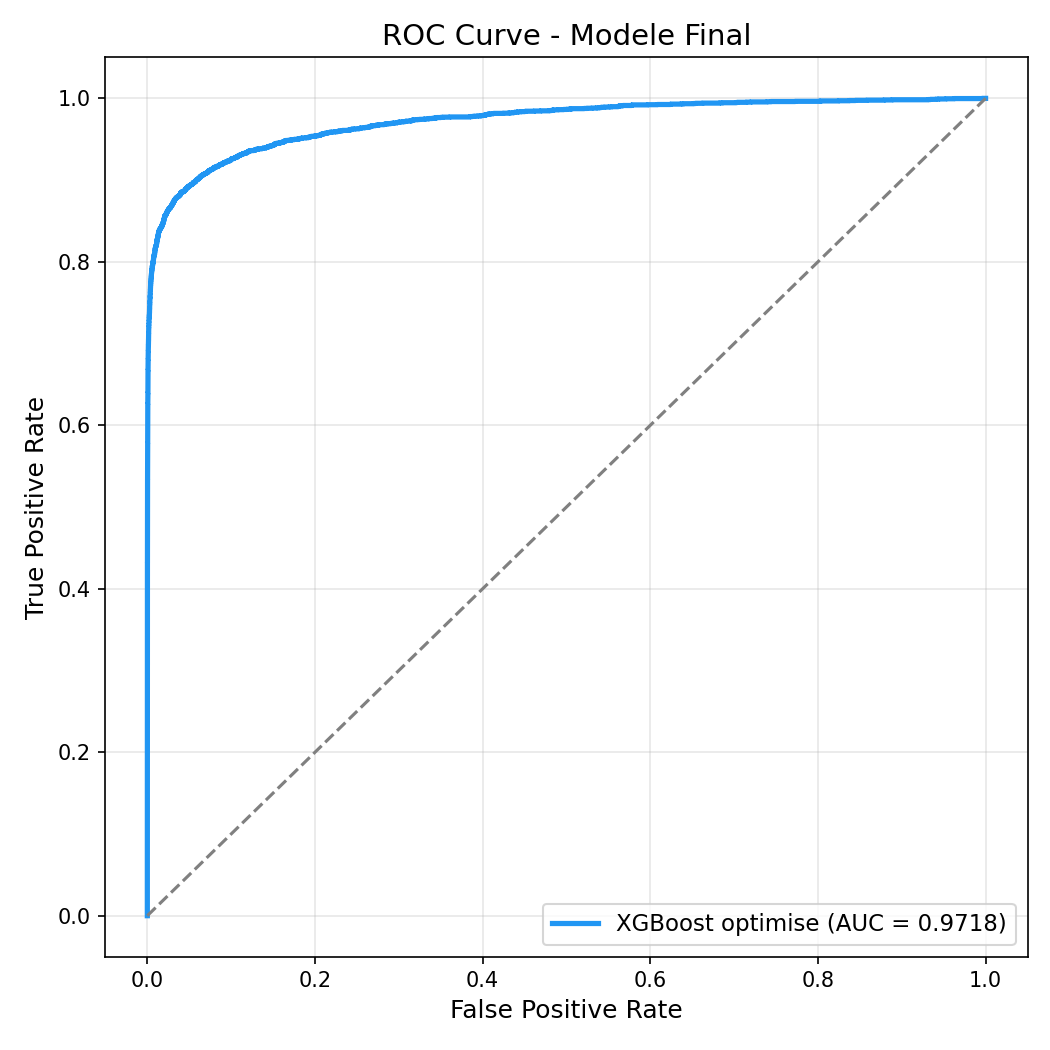
\includegraphics[width=0.85\textwidth]{capstone-ssl-fraud-detection/reports/figures/final_roc.png}
\caption{Courbe ROC du modele final}
\label{fig:roc-final}
\end{figure}

\begin{figure}[H]
\centering
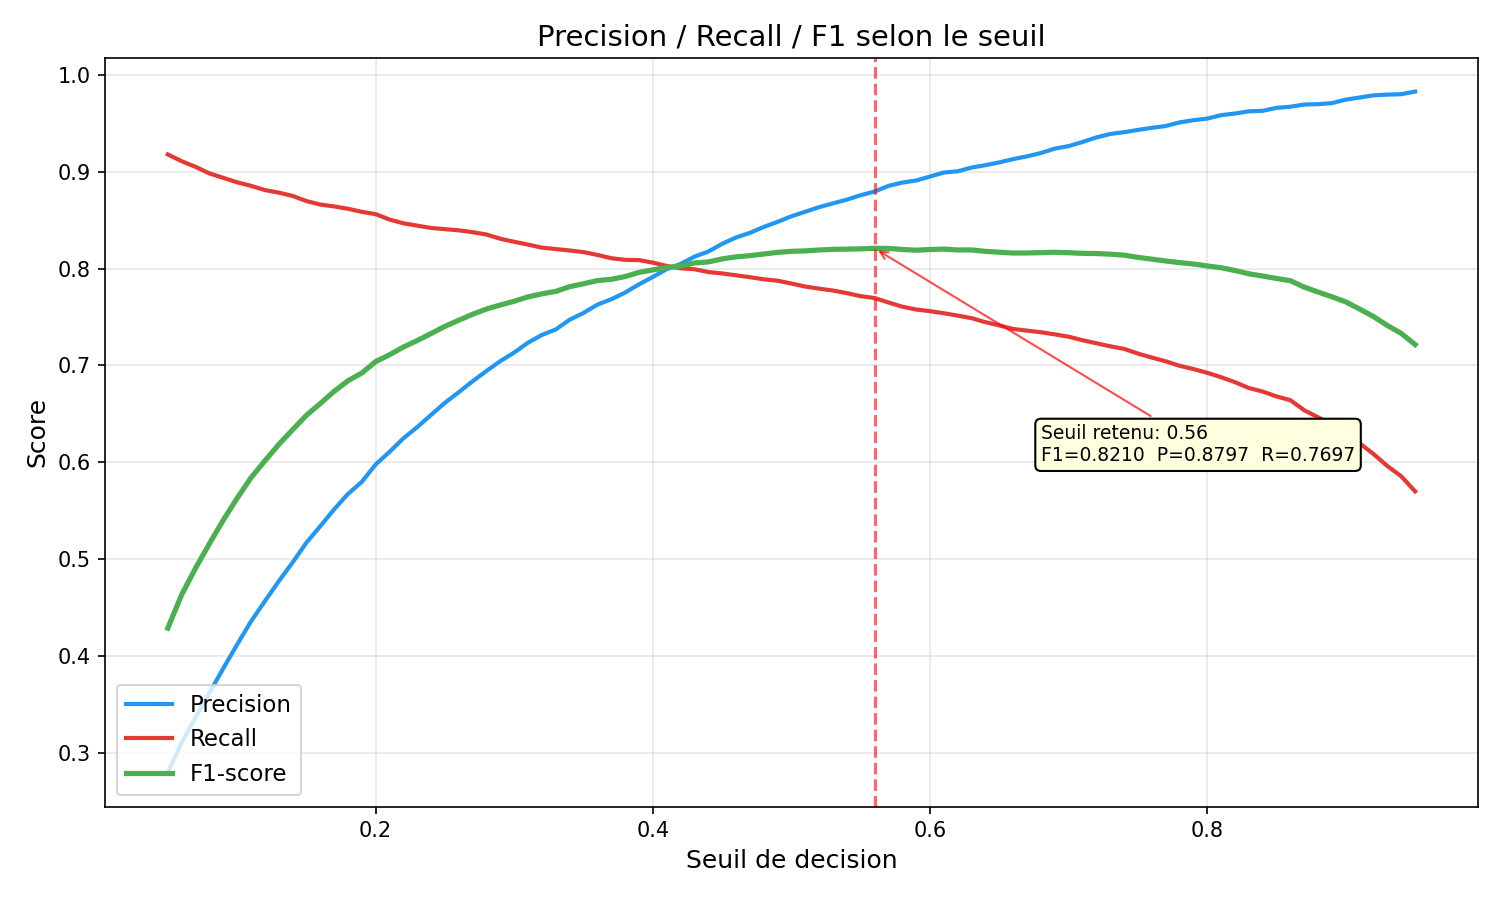
\includegraphics[width=0.85\textwidth]{capstone-ssl-fraud-detection/reports/figures/final_threshold_analysis.png}
\caption{Analyse du seuil de decision}
\label{fig:threshold-final}
\end{figure}

\begin{figure}[H]
\centering
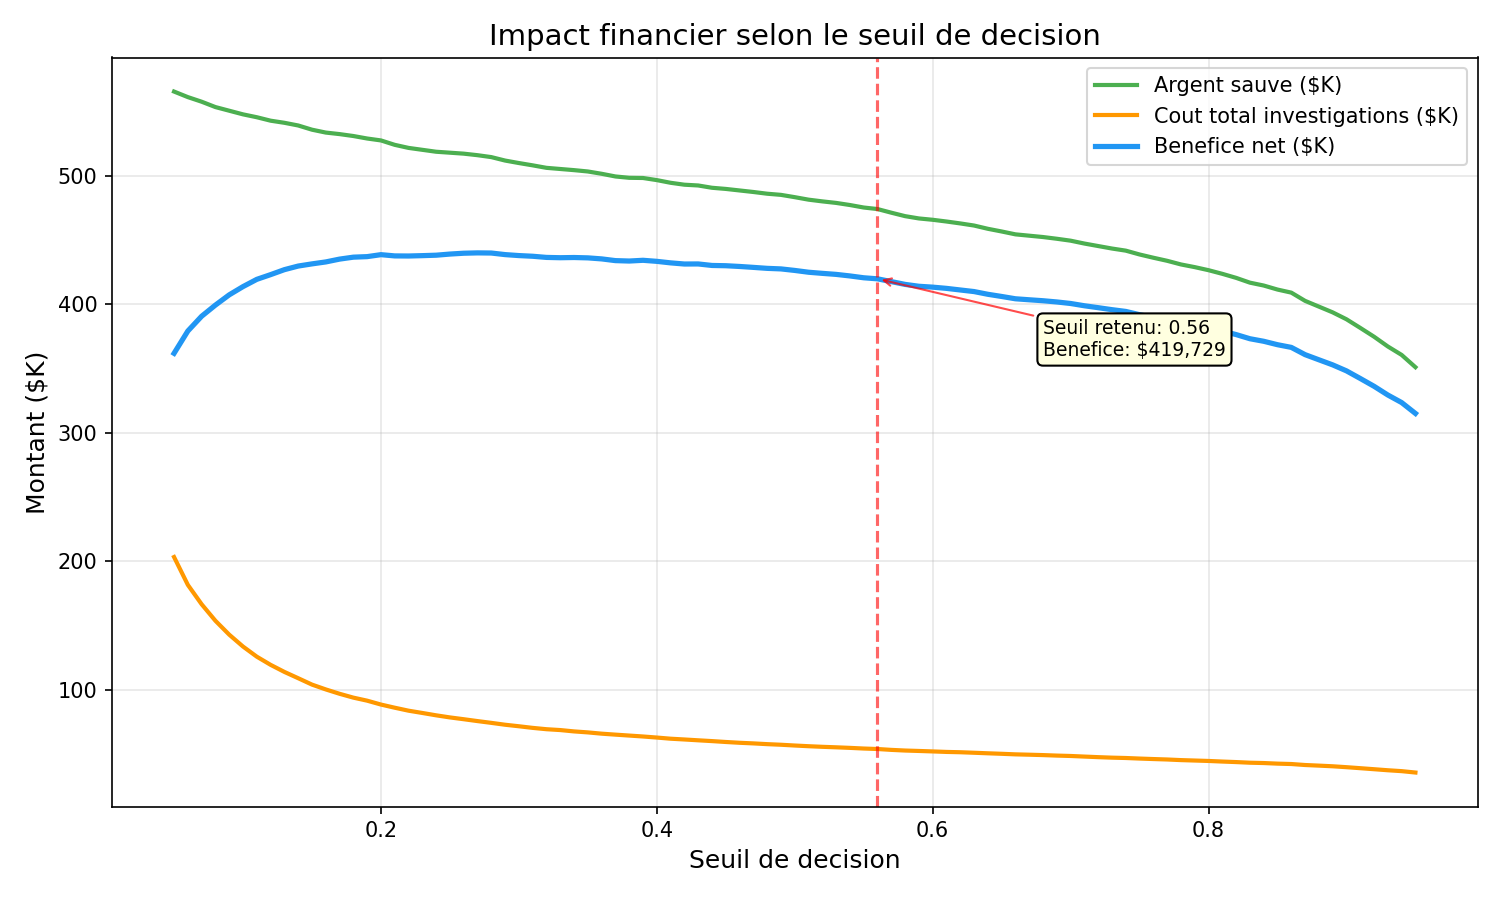
\includegraphics[width=0.85\textwidth]{capstone-ssl-fraud-detection/reports/figures/final_business_impact.png}
\caption{Impact financier du modele final}
\label{fig:business-impact}
\end{figure}

\section{Interpretation metier des resultats}

D'un point de vue bancaire, les metriques finales sont exploitables. Une precision elevee reduit la charge inutile des equipes d'investigation, car les alertes sont majoritairement pertinentes. Un recall de 77\% signifie que le modele detecte une part importante des fraudes, tout en conservant un volume d'alertes raisonnable.

Le modele n'est donc pas seulement performant techniquement. Il est compatible avec une logique operationnelle : identifier les transactions les plus risquees, prioriser les analyses et reduire l'impact financier de la fraude.

% =========================================================
% CHAPITRE 6
% =========================================================
\chapter{KPIs business et impact financier}

\section{Pourquoi traduire les metriques en KPIs}

Dans un projet Data Science in Business, les metriques techniques ne suffisent pas. Un AUC ou un F1-score permet de comparer des modeles, mais ne dit pas directement ce que gagne une banque. Il est donc necessaire de traduire les performances en indicateurs metier : nombre de fraudes detectees, cout des fausses alertes, montant sauve et benefice net.

\section{KPIs globaux du dataset}

\begin{table}[H]
\centering
\caption{KPIs globaux de fraude}
\begin{tabular}{lc}
\toprule
\textbf{Indicateur} & \textbf{Valeur} \\
\midrule
Nombre total de transactions & 590 540 \\
Nombre de fraudes & 20 663 \\
Taux de fraude & 3,50\% \\
Volume frauduleux & 3 083 845 USD \\
Montant moyen d'une fraude & 149,24 USD \\
\bottomrule
\end{tabular}
\end{table}

\section{Analyse par produit}

L'analyse par produit montre une distinction essentielle entre taux de fraude et volume de fraude. Le produit C presente le taux de fraude le plus eleve, avec 11,69\%. Le produit W presente le taux le plus faible, avec 2,04\%, mais il concentre le plus grand volume de transactions. Il genere donc un nombre important de fraudes en valeur absolue.

\begin{table}[H]
\centering
\caption{Fraude par produit}
\begin{tabular}{lccc}
\toprule
\textbf{Produit} & \textbf{Transactions} & \textbf{Fraudes} & \textbf{Taux de fraude} \\
\midrule
C & 68 519 & 8 008 & 11,69\% \\
S & 11 628 & 686 & 5,90\% \\
H & 33 024 & 1 574 & 4,77\% \\
R & 37 699 & 1 426 & 3,78\% \\
W & 439 670 & 8 969 & 2,04\% \\
\bottomrule
\end{tabular}
\end{table}

\begin{figure}[H]
\centering
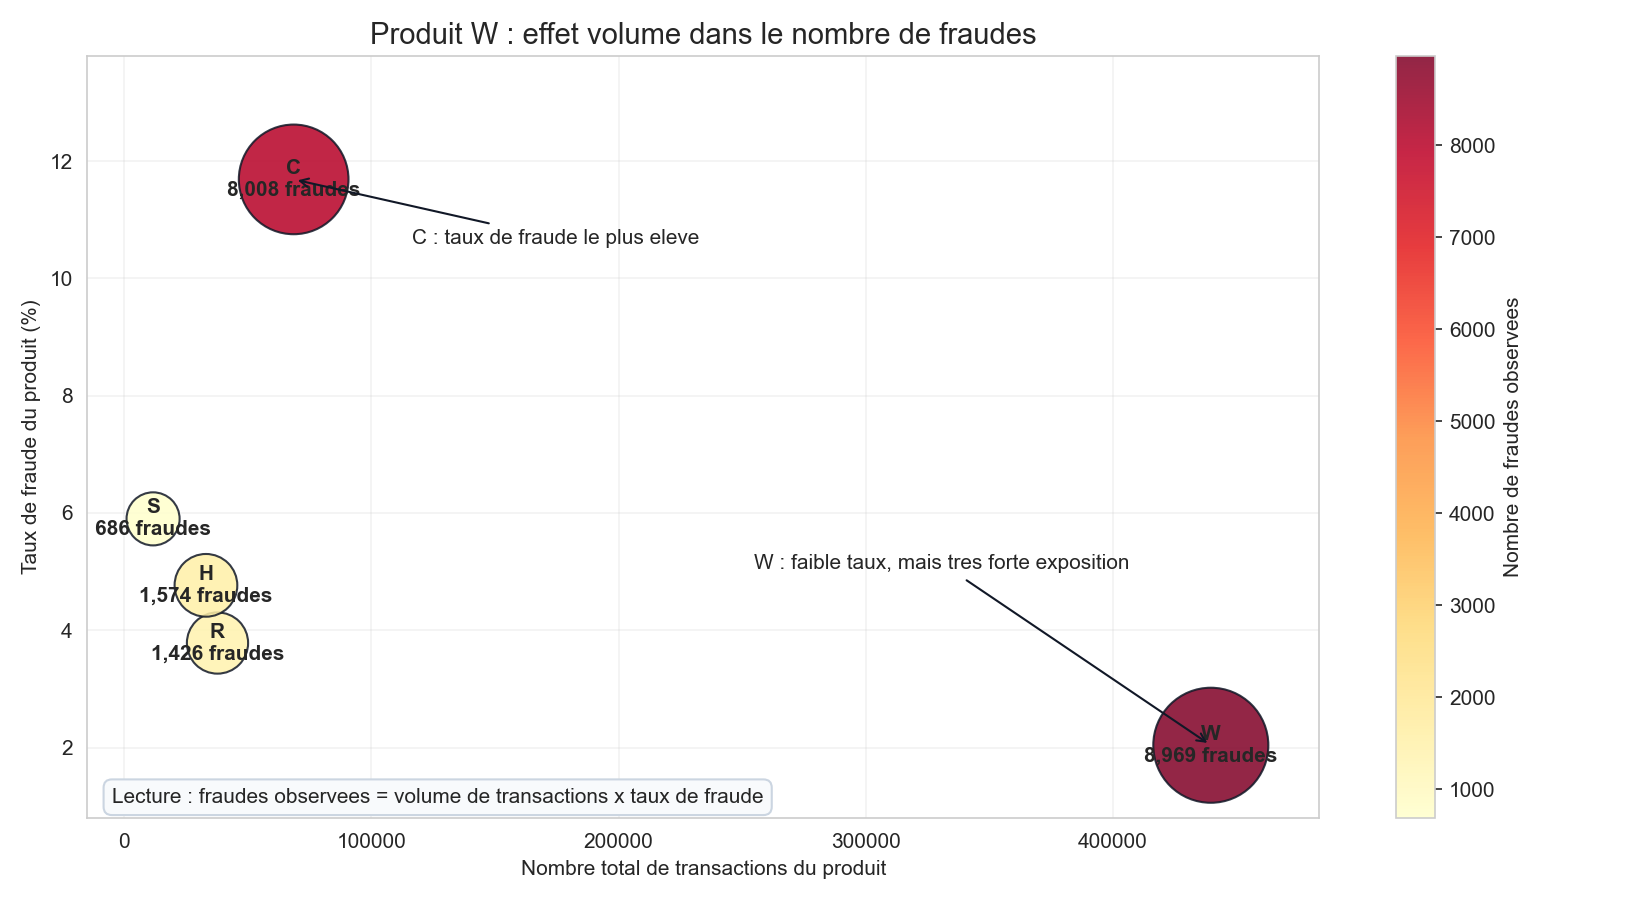
\includegraphics[width=0.9\textwidth]{capstone-ssl-fraud-detection/reports/figures/business_produits_exposition.png}
\caption{Exposition produit : taux de fraude et volume}
\label{fig:product-exposure}
\end{figure}

Cette figure est importante pour la soutenance. Elle permet d'expliquer pourquoi un produit peut avoir un faible taux de fraude mais un volume eleve de fraudes. Le risque relatif et le risque absolu ne racontent pas la meme chose. Pour une banque digitale, les deux lectures sont necessaires.

\section{Impact financier du modele}

En projetant les performances du modele final sur l'ensemble du dataset, les indicateurs metier estimes sont les suivants :

\begin{table}[H]
\centering
\caption{Impact financier estime du modele}
\begin{tabular}{lc}
\toprule
\textbf{Indicateur} & \textbf{Valeur} \\
\midrule
Fraudes detectees estimees & 15 904 / 20 663 \\
Fausses alertes estimees & 2 174 \\
Montant sauve estime & 2 373 635 USD \\
Cout d'investigation estime & 271 170 USD \\
Benefice net estime & 2 102 465 USD \\
\bottomrule
\end{tabular}
\end{table}

Ces chiffres donnent du sens aux metriques ML. Le modele permet non seulement de detecter des fraudes, mais aussi de generer une valeur economique nette. L'estimation du benefice net permet de relier la performance algorithmique a la decision business.

\section{Analyse des fraudes ratees}

Les fraudes ratees par le modele ne doivent pas etre interpretees comme de simples erreurs aleatoires. Leur analyse montre qu'elles ressemblent davantage aux transactions legitimes : elles sont souvent associees au produit W, a des cartes debit, a des domaines email courants et a moins de signaux device distinctifs.

Cette analyse permet de formuler une limite operationnelle : le modele detecte efficacement les fraudes atypiques, mais les fraudes qui imitent fortement les comportements normaux restent plus difficiles. Pour reduire davantage ces faux negatifs, il faudrait enrichir les donnees avec des informations comportementales supplementaires : historique client, geolocalisation, adresse IP, empreinte device, comportement de navigation ou signaux d'authentification.

% =========================================================
% CHAPITRE 7
% =========================================================
\chapter{Dashboard Streamlit et assistant metier}

\section{Objectif du dashboard}

Le dashboard Streamlit a ete developpe pour rendre les resultats accessibles et exploitables. Il permet de passer d'un projet purement technique a une solution demonstrable devant un jury ou un acteur metier. L'interface centralise les metriques finales, les KPIs business, les graphiques explicatifs et un module de test transactionnel.

L'application est disponible a l'adresse suivante :

\begin{center}
\url{https://fraud-detection-bank-ssl.streamlit.app}
\end{center}

\section{Pages principales}

Le dashboard contient plusieurs pages. La vue d'ensemble presente la problematique, les metriques finales et le pipeline global. La page Exploration permet de visualiser le dataset et son desequilibre. La page KPIs Business presente les indicateurs metier, les graphiques produits, l'impact financier et l'exposition transactionnelle. La page Test du modele permet de simuler une transaction. La page Performances presente les resultats du modele final et les hyperparametres de maniere lisible. Enfin, la page Assistant metier integre un chatbot local.

\section{Interface de test transactionnel}

La page de test permet a l'utilisateur de saisir des caracteristiques de transaction : montant, produit, heure, type de carte, reseau, email et device. Le dashboard renvoie un score de risque et des facteurs explicatifs. Cette interface ne remplace pas le scoring complet XGBoost sur les 743 variables, mais elle permet de vulgariser la logique du modele et de montrer les facteurs de risque detectes.

\section{Assistant metier}

L'assistant metier a ete concu comme un chatbot local integre au dashboard. Son role est de repondre aux questions sur le projet, les metriques, le seuil, les KPIs, le produit W, le SSL et les recommandations metier. Il ne doit pas inventer des resultats : ses reponses sont basees sur les rapports et les constantes validees du projet.

L'assistant couvre cinq piliers :

\begin{enumerate}
    \item analyse conversationnelle de transaction ;
    \item questions sur les resultats du projet ;
    \item explication des KPIs ;
    \item recommandations metier ;
    \item simulation de scenarios.
\end{enumerate}

\section{Interet pour la soutenance}

Le dashboard constitue un support fort pour la soutenance. Il permet de montrer que le projet n'est pas seulement un entrainement de modele, mais une solution complete. Le jury peut visualiser les resultats, tester des scenarios et comprendre les arbitrages metier.

% =========================================================
% CHAPITRE 8
% =========================================================
\chapter{Architecture technique et implementation}

\section{Organisation generale du projet}

Le projet a ete organise de maniere modulaire afin de separer les donnees, les scripts, les modeles, les resultats et l'application. Cette organisation repond a un objectif de reproductibilite : chaque etape du pipeline peut etre relancee et verifiee independamment.

La structure principale comprend un dossier `data` pour les donnees brutes et traitees, un dossier `src` pour les scripts Python, un dossier `models` pour les modeles sauvegardes, un dossier `reports` pour les resultats et les figures, ainsi qu'un fichier `app\_dashboard.py` pour l'application Streamlit. Cette separation permet de distinguer les artefacts de calcul des artefacts de restitution.

\begin{table}[H]
\centering
\caption{Organisation des principaux dossiers}
\begin{tabular}{p{4cm}p{10cm}}
\toprule
\textbf{Dossier/Fichier} & \textbf{Role} \\
\midrule
data/raw & Donnees brutes issues du dataset IEEE-CIS. \\
data/processed & Donnees nettoyees et transformees au format Parquet. \\
src & Scripts de preprocessing, entrainement, evaluation et optimisation. \\
models & Modeles entraines et sauvegardes. \\
reports/results & Rapports texte, predictions et metriques. \\
reports/figures & Graphiques generes pour le dashboard et le memoire. \\
app\_dashboard.py & Application Streamlit deployee. \\
\bottomrule
\end{tabular}
\end{table}

\section{Pipeline d'execution}

Le pipeline suit une logique sequentielle. Les fichiers bruts sont d'abord charges et transformes. Les donnees traitees sont ensuite utilisees pour entrainer les modeles. Les predictions sont sauvegardees afin de produire les metriques, les graphiques et les analyses business. Enfin, le dashboard lit ces artefacts pour presenter les resultats.

Cette logique evite de recalculer inutilement les modeles dans l'application Streamlit. Le dashboard ne doit pas entrainer un modele a chaque ouverture. Il doit charger les resultats valides et les visualiser. Cette separation entre calcul et restitution est essentielle pour un deploiement stable.

\section{Choix technologiques}

Python a ete utilise comme langage principal pour l'ensemble du projet. Pandas et NumPy ont servi a la manipulation des donnees. Scikit-learn a ete utilise pour les metriques, le split stratifie et certaines routines d'evaluation. XGBoost a ete retenu pour le modele final. Plotly et Matplotlib ont servi a la generation des figures, tandis que Streamlit a ete utilise pour le dashboard.

Le choix de Streamlit est coherent avec un projet capstone : il permet de produire rapidement une interface interactive, de partager les resultats et de rendre le modele comprehensible par un public non technique. Dans une architecture industrielle, une application plus robuste pourrait etre developpee avec une API backend, une base de donnees et un systeme d'authentification. Pour le perimetre du projet, Streamlit offre un bon compromis entre rapidite, pedagogie et demonstration.

\section{Gestion des gros fichiers}

Les fichiers du dataset sont volumineux. Pour permettre le deploiement et la collaboration via GitHub, les donnees ont ete versionnees avec Git LFS. Cette decision permet de conserver les donnees dans le depot tout en evitant les limites classiques de Git sur les gros fichiers.

Cependant, le deploiement cloud a revele une contrainte importante : charger directement de tres gros CSV peut provoquer des erreurs ou des lenteurs. Une correction a donc ete apportee dans le dashboard pour charger uniquement les colonnes necessaires aux KPIs business et utiliser des valeurs de secours validees par les rapports si les fichiers bruts ne sont pas disponibles. Cette correction montre l'importance de penser la robustesse de l'application, et pas seulement les performances du modele.

\section{Reproductibilite}

La reproductibilite repose sur trois elements : les scripts, les donnees traitees et les rapports generes. Chaque resultat important du memoire doit pouvoir etre relie a un script ou a un fichier de sortie. Les metriques finales proviennent du script d'optimisation des hyperparametres, les KPIs metier proviennent des analyses business, et les figures proviennent du dossier `reports/figures`.

Pour une version finale, il est recommande d'ajouter un fichier `README` plus detaille, listant l'ordre d'execution exact, les dependances et les commandes de reproduction. Cette recommandation figure egalement dans les perspectives operationnelles.

% =========================================================
% CHAPITRE 9
% =========================================================
\chapter{Discussion critique}

\section{Lecture scientifique des resultats}

Les resultats du projet peuvent etre lus selon deux niveaux. Le premier niveau concerne la performance finale du modele. De ce point de vue, le XGBoost optimise donne des resultats solides, avec une AUC-ROC de 0,9718 et un F1-score de 0,8210. Ces chiffres indiquent que le pipeline final est capable d'identifier efficacement les transactions frauduleuses dans un dataset fortement desequilibre.

Le second niveau concerne l'hypothese initiale autour du self-supervised learning. Le projet a montre que le SSL ne surpasse pas XGBoost sur ce dataset tabulaire. Cette conclusion ne doit pas etre interpretee comme un echec, mais comme un resultat scientifique. Elle montre que les methodes de representation learning ne sont pas automatiquement superieures sur toutes les formes de donnees. Dans les donnees tabulaires, les variables sont deja structurees, et les modeles a arbres peuvent exploiter directement les interactions pertinentes.

\section{Pourquoi le SSL reste valorisable}

Le SSL reste important dans la demarche du projet pour trois raisons. Premierement, il a permis de tester une hypothese coherente avec la problematique des labels rares. Deuxiemement, il a structure une demarche experimentale comparative entre apprentissage non supervise, semi-supervise et supervise. Troisiemement, il a permis de montrer que le choix final du modele n'est pas arbitraire : XGBoost a ete retenu parce qu'il a ete compare a d'autres approches.

Dans le memoire, il faut donc presenter le SSL comme une composante exploratoire et scientifique de la demarche, et non comme le modele final. Le systeme final est hybride au sens methodologique : exploration SSL, apprentissage supervise XGBoost, optimisation metier et restitution dashboard.

\section{Equilibre entre performance et exploitabilite}

Un modele de fraude ne peut pas etre juge uniquement sur une metrique globale. Une banque digitale doit arbitrer entre la detection des fraudes et la limitation des fausses alertes. Un recall tres eleve peut sembler attractif, mais il peut generer un volume d'alertes impossible a traiter. Une precision tres elevee peut reduire la charge operationnelle, mais laisser passer trop de fraudes.

Le seuil final de 0,56 a ete retenu car il donne un compromis coherent apres optimisation du modele. Il detecte environ 77\% des fraudes avec environ 88\% de precision. Cette configuration est defendable dans une logique metier : le modele signale des alertes de qualite tout en detectant une part importante des fraudes.

\section{Analyse du produit W}

Le cas du produit W illustre l'importance de distinguer taux et volume. Le produit W a le taux de fraude le plus faible, mais il genere le plus grand nombre de fraudes en valeur absolue car il represente la majorite des transactions. Cette observation est essentielle pour une banque digitale. Une strategie antifraude ne doit pas uniquement surveiller les segments a taux de fraude eleve ; elle doit aussi surveiller les segments a forte exposition.

Le produit C, avec un taux de fraude de 11,69\%, doit etre considere comme un produit a risque relatif eleve. Le produit W, avec un taux de 2,04\% mais un volume tres important, doit etre considere comme un produit a risque absolu significatif. Cette double lecture permet de mieux orienter les controles.

\section{Limites liees au dataset}

Le dataset IEEE-CIS est riche, mais il presente des limites. Certaines variables sont anonymisees, ce qui limite l'interpretation fine. Les donnees ne representent pas un flux temps reel complet. Le label fraude est disponible pour l'entrainement, mais le processus exact d'investigation ayant produit ce label n'est pas detaille. Enfin, le dataset ne contient pas toutes les informations qu'une banque pourrait utiliser en production, comme l'historique complet du client, l'adresse IP, la geolocalisation precise ou les signaux comportementaux.

Ces limites n'invalident pas le projet. Elles permettent au contraire de formuler des perspectives realistes. Le modele actuel est performant sur les donnees disponibles, mais une version industrielle devrait etre enrichie par des donnees supplementaires et un suivi temporel.

\section{Limites liees au deploiement}

Le dashboard Streamlit est une interface de demonstration et d'aide a la comprehension. Il ne constitue pas une architecture bancaire de production. Dans un environnement reel, il faudrait separer le moteur de scoring, l'API de prediction, la base de donnees transactionnelle, les droits utilisateurs, la journalisation et le monitoring. Il faudrait aussi garantir la securite, la tracabilite et la conformite reglementaire.

Le dashboard reste toutefois parfaitement adapte au cadre du capstone. Il demontre la capacite a rendre le modele accessible, a visualiser les KPIs et a expliquer les decisions.

\section{Apport pour une banque digitale}

L'apport principal du projet est de proposer une chaine coherente de detection de fraude. Cette chaine commence par les donnees, passe par le modele, se poursuit par le choix du seuil, puis aboutit a des KPIs et a un dashboard. Elle permet a une banque digitale de comprendre non seulement quelles transactions sont suspectes, mais aussi pourquoi elles le sont et quel impact financier peut etre attendu.

Cette approche est plus utile qu'un simple modele isole. Elle transforme une prediction en decision. Elle rend le projet compatible avec les attentes d'un service risque, d'une equipe data et d'une direction metier.

% =========================================================
% CHAPITRE 10
% =========================================================
\chapter{Preconisations operationnelles}

\section{Mettre en place une strategie de scoring}

La premiere recommandation est d'utiliser le modele XGBoost optimise comme systeme de scoring transactionnel. Chaque transaction recoit un score de risque. Ce score doit ensuite etre transforme en decision selon un seuil metier. Le seuil final de 0,56 constitue un bon compromis sur les donnees de validation.

\section{Adopter une logique de priorisation}

Toutes les alertes ne doivent pas etre traitees de la meme maniere. Les transactions avec les scores les plus eleves doivent etre priorisees par les equipes d'investigation. Une banque digitale peut ainsi organiser son traitement en trois niveaux : autorisation automatique pour les faibles risques, revue manuelle pour les cas intermediaires et blocage ou verification renforcee pour les risques eleves.

\section{Surveiller les produits a risque}

Le produit C presente un taux de fraude eleve. Il doit faire l'objet d'une surveillance renforcee. Le produit W, en revanche, presente un faible taux relatif mais un volume de fraude important. La banque doit donc distinguer deux logiques : les produits a fort taux de risque et les produits a forte exposition volumique.

\section{Suivre les KPIs dans le temps}

Le modele doit etre accompagne d'un suivi regulier. Les KPIs a suivre incluent le taux de fraude, le nombre d'alertes, la precision des alertes, le recall estime, le cout d'investigation, le montant sauve et le benefice net. Ce suivi permet de detecter une degradation du modele ou une evolution des strategies de fraude.

\section{Enrichir les donnees}

Pour ameliorer la detection des fraudes difficiles, il est recommande d'ajouter des signaux comportementaux. Les donnees actuelles sont riches, mais certaines fraudes ratees imitent fortement les transactions legitimes. Des informations telles que l'historique client, l'adresse IP, la geolocalisation, l'empreinte device ou le comportement de navigation pourraient ameliorer la separation entre fraude et legitimite.

\section{Maintenir l'explicabilite}

Une banque digitale ne peut pas deployer un modele totalement opaque sans cadre de controle. Il est donc recommande d'ajouter des outils d'explicabilite tels que SHAP afin d'expliquer localement les decisions du modele. Cette piste est importante pour l'acceptation par les equipes metier et pour la gouvernance du risque.

% =========================================================
% CONCLUSION
% =========================================================
\chapter{Conclusion}

Ce memoire a presente une demarche complete de detection de fraude dans un contexte de banque digitale. La problematique portait sur la conception d'un systeme hybride combinant self-supervised learning, apprentissage supervise et optimisation metier afin d'ameliorer la performance, l'explicabilite et l'exploitabilite des decisions dans un contexte de donnees desequilibrees.

La demarche a commence par une analyse du dataset IEEE-CIS Fraud Detection et par la mise en place d'un ETL leger. Deux versions de preprocessing ont ete construites. La premiere a permis d'obtenir une base exploitable, mais a revele des limites liees a la suppression trop forte de variables. La deuxieme a conserve davantage d'information, ajoute des indicateurs de valeurs manquantes et integre des features metier.

Le self-supervised learning a ete teste comme approche exploratoire. Les resultats ont montre que, dans ce contexte tabulaire, les representations SSL n'apportaient pas de gain significatif par rapport a un modele XGBoost supervise. Cette conclusion est importante : elle montre que le projet ne s'est pas limite a valider une hypothese initiale, mais a confronte cette hypothese aux resultats experimentaux.

Le modele final retenu est un XGBoost optimise. Il atteint une AUC-ROC de 0,9718, une Average Precision de 0,8608, un F1-score de 0,8210, une precision de 0,8797 et un recall de 0,7697. Ces resultats montrent une performance robuste dans un contexte fortement desequilibre. Le seuil final de 0,56 permet un compromis coherent entre detection de fraude et controle des fausses alertes.

La contribution principale du projet reside dans la transformation de ces resultats techniques en lecture business. Le modele permet d'estimer un benefice net de 2 102 465 USD, apres prise en compte du montant sauve et du cout d'investigation. Le dashboard Streamlit rend ces resultats accessibles, visualisables et testables. Il permet de presenter le projet comme un systeme d'aide a la decision et non comme un simple modele de classification.

Les limites principales concernent la nature du dataset, l'absence de donnees comportementales historiques et la difficulte a detecter certaines fraudes qui imitent les transactions legitimes. Les perspectives portent sur l'ajout de donnees temps reel, l'explicabilite locale, le monitoring du drift et l'integration dans une architecture bancaire de production.

En conclusion, ce projet illustre l'esprit Data Science in Business : mobiliser des donnees, des algorithmes et des indicateurs metier pour repondre a un probleme professionnel concret. La detection de fraude n'est pas uniquement une question de score, mais une question d'arbitrage, de cout, d'interpretation et de decision.

% =========================================================
% BIBLIOGRAPHIE
% =========================================================
\begin{thebibliography}{99}
\addcontentsline{toc}{chapter}{Bibliographie}

\bibitem{dataset}
Kaggle. IEEE-CIS Fraud Detection. Disponible sur : \url{https://www.kaggle.com/c/ieee-fraud-detection}. Consulte le 23 juin 2026.

\bibitem{lucas2020survey}
Lucas, Y. et Jurgovsky, J. (2020). Credit card fraud detection using machine learning: A survey. arXiv:2010.06479. Disponible sur : \url{https://arxiv.org/abs/2010.06479}.

\bibitem{saito2015pr}
Saito, T. et Rehmsmeier, M. (2015). The Precision-Recall Plot Is More Informative than the ROC Plot When Evaluating Binary Classifiers on Imbalanced Datasets. PLOS ONE, 10(3). Disponible sur : \url{https://doi.org/10.1371/journal.pone.0118432}.

\bibitem{deng2019fraudjudger}
Deng, R. et Ruan, N. (2019). FraudJudger: Real-World Data Oriented Fraud Detection on Digital Payment Platforms. arXiv:1909.02398. Disponible sur : \url{https://arxiv.org/abs/1909.02398}.

\bibitem{han2026cfa}
Han, X. et Wu, C. (2026). Validation-Stage Combinatorial Fusion Analysis for Imbalanced Credit-Card Fraud Detection. arXiv:2606.10393. Disponible sur : \url{https://arxiv.org/abs/2606.10393}.

\bibitem{pstb}
PST\&B. Site officiel Paris School of Technology \& Business. Disponible sur : \url{https://www.pstb.fr/}. Consulte le 23 juin 2026.

\bibitem{xgboost}
Chen, T. et Guestrin, C. (2016). XGBoost: A Scalable Tree Boosting System. Proceedings of the 22nd ACM SIGKDD International Conference on Knowledge Discovery and Data Mining.

\end{thebibliography}

% =========================================================
% ANNEXES
% =========================================================
\appendix

\chapter{Annexe A - Hyperparametres finaux}

\begin{longtable}{lc}
\caption{Hyperparametres du modele XGBoost final}\\
\toprule
\textbf{Hyperparametre} & \textbf{Valeur} \\
\midrule
colsample\_bytree & 0,7364265404201034 \\
gamma & 0,056736760620294535 \\
learning\_rate & 0,14870404274178442 \\
max\_depth & 9 \\
min\_child\_weight & 3 \\
n\_estimators & 562 \\
reg\_alpha & 0,659984046034179 \\
reg\_lambda & 2,1344444004024314 \\
subsample & 0,822080324639785 \\
\bottomrule
\end{longtable}

\chapter{Annexe B - Figures complementaires}

\begin{figure}[H]
\centering
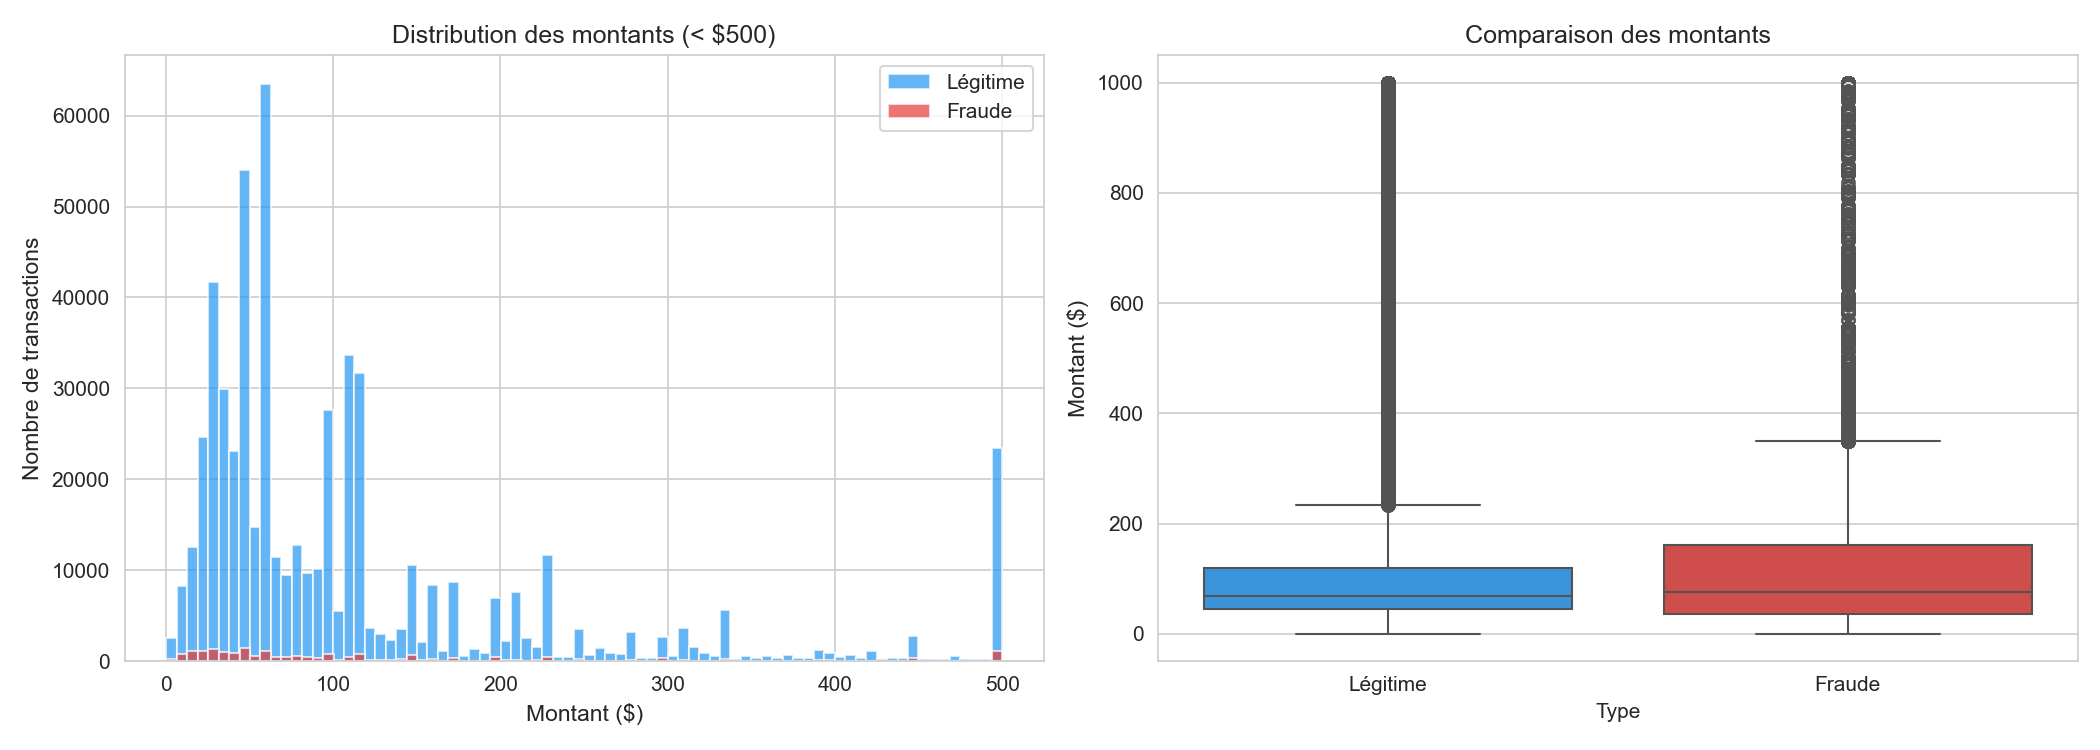
\includegraphics[width=0.9\textwidth]{capstone-ssl-fraud-detection/reports/figures/business_montants.png}
\caption{Distribution des montants et impact metier}
\end{figure}

\begin{figure}[H]
\centering
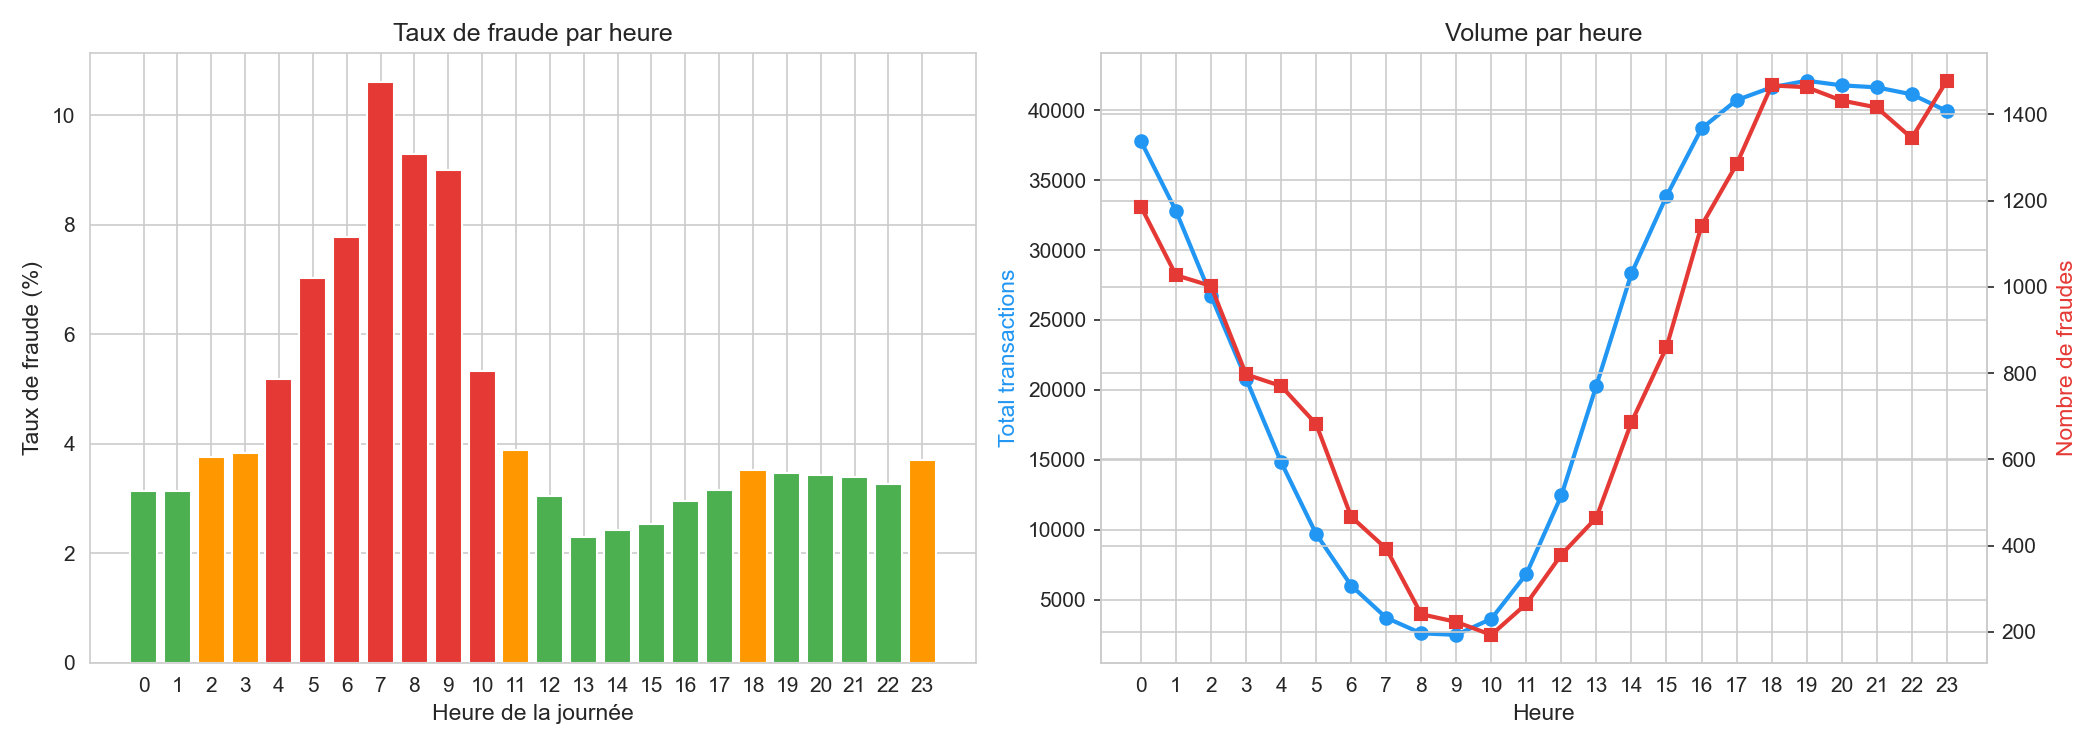
\includegraphics[width=0.9\textwidth]{capstone-ssl-fraud-detection/reports/figures/business_temporel.png}
\caption{Analyse temporelle de la fraude}
\end{figure}

\begin{figure}[H]
\centering
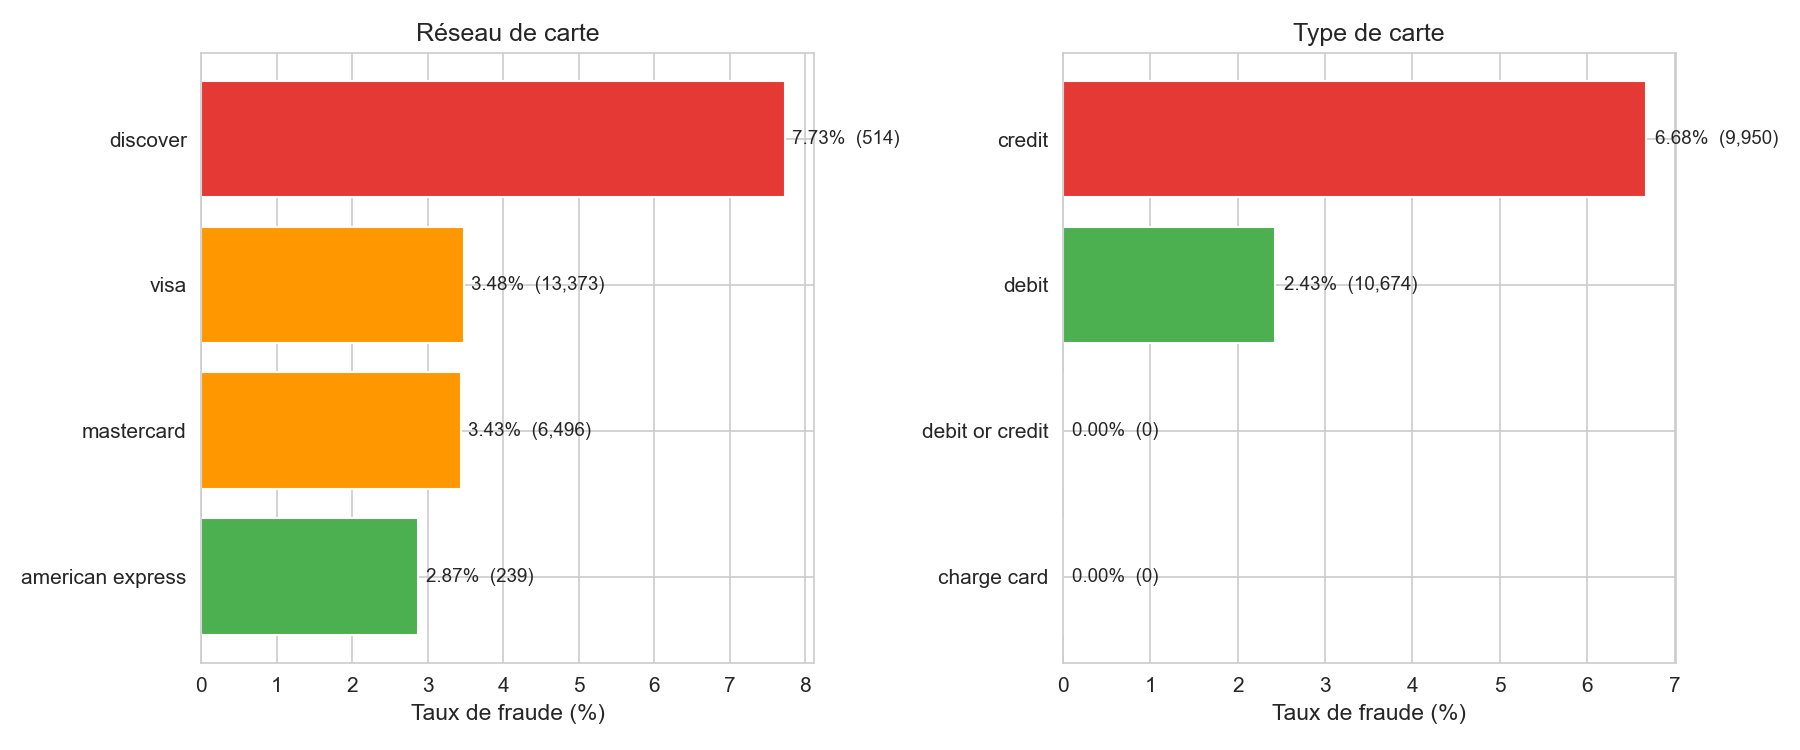
\includegraphics[width=0.9\textwidth]{capstone-ssl-fraud-detection/reports/figures/business_cartes.png}
\caption{Risque par type de carte}
\end{figure}

\begin{figure}[H]
\centering
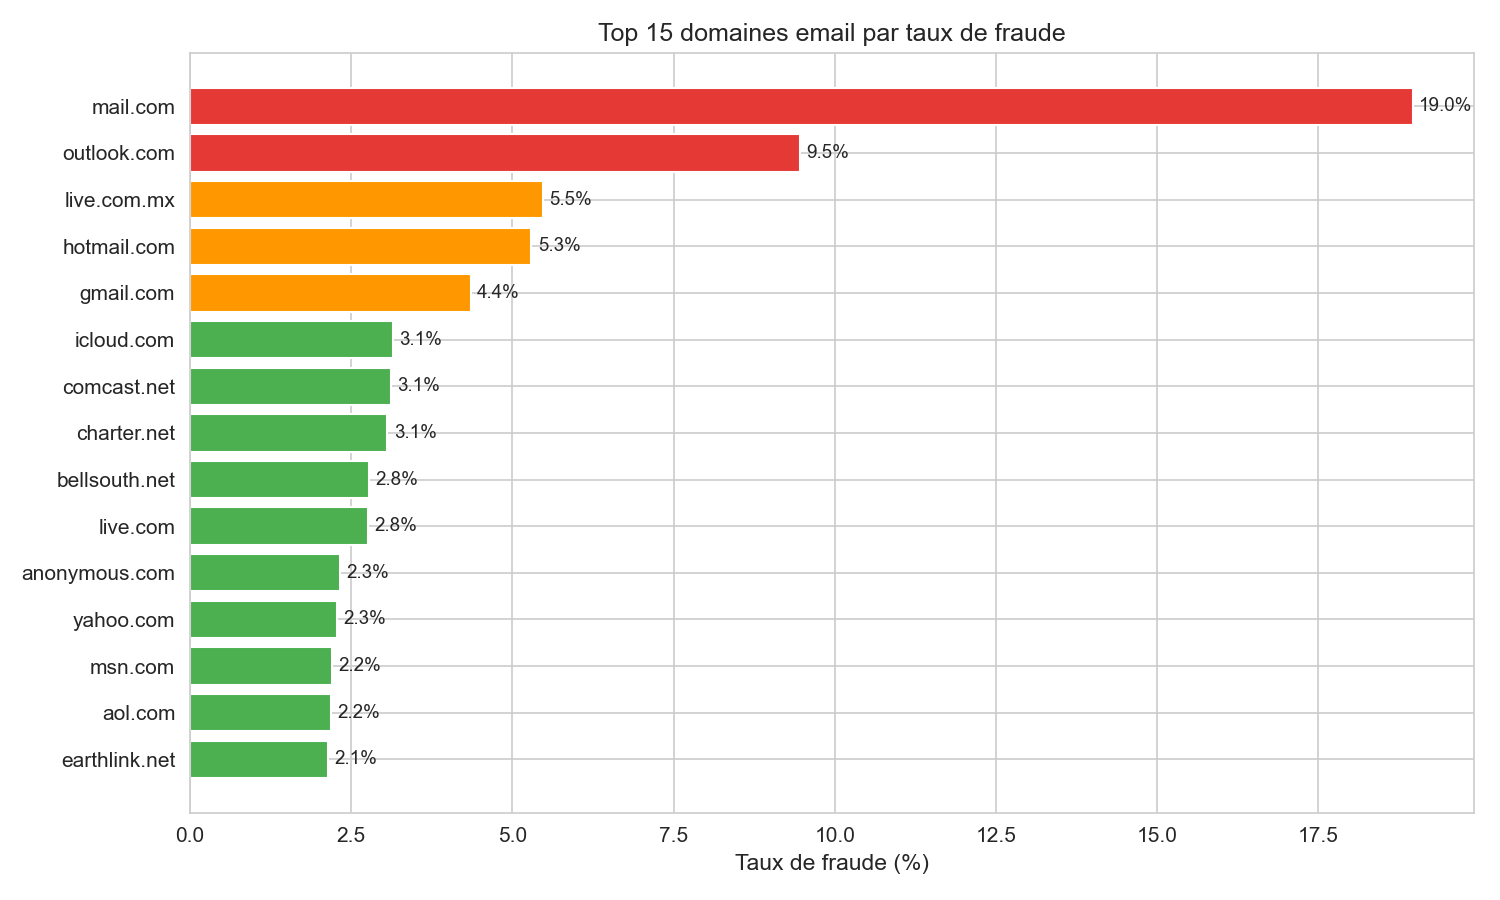
\includegraphics[width=0.9\textwidth]{capstone-ssl-fraud-detection/reports/figures/business_emails.png}
\caption{Risque par domaine email}
\end{figure}

\chapter{Annexe C - Commandes principales}

\begin{verbatim}
python src/data_preprocessing_v2.py
python src/train_ssl.py
python src/hybrid_xgboost.py
python src/hyperparameter_tuning.py
streamlit run capstone-ssl-fraud-detection/app_dashboard.py
\end{verbatim}

\chapter{Annexe D - Architecture du dashboard}

Le dashboard est organise autour de six modules : vue d'ensemble, exploration des donnees, KPIs business, test du modele, performances et assistant metier. Cette architecture permet de couvrir les besoins d'un jury technique comme d'un acteur metier.

\chapter{Annexe E - Utilisation d'outils d'IA generative}

Des outils d'IA generative ont ete utilises comme assistance a la structuration, a la reformulation et a la verification de coherence du projet. Les resultats, metriques, donnees et graphiques presentes dans ce memoire proviennent des scripts executes dans le projet et des rapports generes localement. L'utilisation de l'IA n'a pas servi a inventer des resultats experimentaux.

\chapter{Annexe F - Chronologie des iterations}

\begin{longtable}{p{2cm}p{4cm}p{5cm}p{4cm}}
\caption{Chronologie synthetique du projet}\\
\toprule
\textbf{Iteration} & \textbf{Objectif} & \textbf{Resultat observe} & \textbf{Decision} \\
\midrule
1 & Setup et comprehension des donnees & Dataset charge, desequilibre identifie, variables nombreuses et manquantes & Construire un ETL leger \\
2 & Preprocessing V1 & Donnees exploitables mais appauvrissement fort & Ameliorer la conservation des variables \\
3 & SSL initial & Reconstruction possible mais classification faible & Corriger le desequilibre \\
4 & Fine-tuning pondere & Recall ameliore mais performance insuffisante & Tester un modele tabulaire fort \\
5 & XGBoost baseline & Meilleure performance que SSL & Optimiser hyperparametres \\
6 & Preprocessing V2 & Environ 743 features conservees et enrichies & Reentrainer les modeles \\
7 & Comparaison SSL / XGBoost & SSL non superieur au modele supervise & Retenir XGBoost pour la decision \\
8 & Optimisation XGBoost & Forte progression des metriques & Retenir le modele final \\
9 & KPIs et dashboard & Resultats traduits en impact metier & Deployer Streamlit \\
\bottomrule
\end{longtable}

\chapter{Annexe G - Questions possibles du jury}

\section*{Pourquoi avoir teste le SSL si XGBoost est final ?}

Le SSL a ete teste parce que la problematique initiale portait sur la rarete potentielle des labels de fraude. Dans un contexte bancaire reel, les labels confirmes dependent souvent d'investigations humaines. Le SSL permet d'exploiter les transactions non labellisees pour apprendre des representations. Les experiments ont montre que, sur ce dataset tabulaire, XGBoost exploite mieux les features disponibles. Cette conclusion est un resultat scientifique et justifie le choix final.

\section*{Pourquoi le dataset IEEE-CIS est-il pertinent pour la banque digitale ?}

Il s'agit d'un dataset transactionnel de grande taille, avec un label fraude, un fort desequilibre et des variables proches d'un contexte de paiement digital : montant, produit, carte, email, temps et identity/device. Il permet donc de traiter a la fois la modelisation et l'interpretation metier.

\section*{Pourquoi ne pas utiliser l'accuracy ?}

L'accuracy est trompeuse dans un dataset desequilibre. Avec 96,5\% de transactions legitimes, un modele qui predit toujours "legitime" aurait une accuracy elevee mais ne detecterait aucune fraude. Les metriques retenues sont donc precision, recall, F1-score, AUC-ROC et PR-AUC.

\section*{Pourquoi le seuil 0,56 ?}

Le seuil 0,56 est le seuil final issu de l'evaluation sur validation apres optimisation. Il donne un compromis fort entre precision et recall, avec une precision de 0,8797 et un recall de 0,7697. Il permet de detecter une part importante des fraudes tout en limitant les fausses alertes.

\section*{Pourquoi le produit W genere-t-il beaucoup de fraudes alors que son taux est faible ?}

Parce que le produit W concentre un tres grand volume de transactions. Son taux de fraude est faible, mais son exposition est massive. En risque bancaire, il faut distinguer le risque relatif, mesure par le taux, et le risque absolu, mesure par le nombre total de fraudes.

\section*{Le dashboard est-il un outil de production ?}

Non, le dashboard est un prototype de restitution et d'aide a la decision. Il montre comment les resultats peuvent etre exploites. Une version industrielle necessiterait une API securisee, une base de donnees transactionnelle, un monitoring, une authentification et une gouvernance de modele.

\chapter{Annexe H - Grille de lecture metier des erreurs}

\begin{longtable}{p{4cm}p{5cm}p{6cm}}
\caption{Interpretation metier des types d'erreurs}\\
\toprule
\textbf{Cas} & \textbf{Signification ML} & \textbf{Impact metier} \\
\midrule
Vrai positif & Fraude correctement detectee & Perte potentielle evitee, transaction a investiguer ou bloquer. \\
Faux positif & Transaction legitime signalee comme fraude & Cout d'investigation, friction client, risque d'insatisfaction. \\
Vrai negatif & Transaction legitime acceptee & Experience client preservee, pas de cout operationnel. \\
Faux negatif & Fraude non detectee & Perte financiere directe et risque de repetition. \\
\bottomrule
\end{longtable}

\chapter{Annexe I - Structure recommandee pour la soutenance}

La soutenance de 15 minutes peut etre organisee ainsi :

\begin{enumerate}
    \item Contexte banque digitale et fraude : 1 minute.
    \item Problematique et objectifs : 1 minute.
    \item Dataset et justification : 2 minutes.
    \item Methodologie : ETL, SSL, XGBoost : 3 minutes.
    \item Resultats modeles : 3 minutes.
    \item KPIs business et impact financier : 2 minutes.
    \item Dashboard et demonstration : 2 minutes.
    \item Conclusion et perspectives : 1 minute.
\end{enumerate}

La partie en anglais peut couvrir l'introduction, le contexte et la revue de litterature. La partie demonstration peut etre realisee en francais pour faciliter l'interaction avec le jury.

\end{document}
